\section{结果}

\subsection{离线均衡器相对传统基线}

先看离线模型的均衡能力。表 1 与图 2 给出 3 seed × 60 帧主矩阵的 Data BER。离线神经均衡器在 0/5/10/15 dB 为 22.19\%/5.96\%/1.06\%/0.216\%；CFO+DD-Phase DFE-RLS 为 44.05\%/18.30\%/6.91\%/4.37\%；LMMSE-FIR 为 44.01\%/22.43\%/7.22\%/5.05\%。相对 DFE-RLS，四个 SNR 的 BER 降低分别为 49.6\%、67.4\%、84.7\%、95.1\%。三个独立 seed 中，每个 SNR 的 Frozen 都低于该传统基线。

\begin{table}[htbp]
\centering
\small
\caption{离线神经均衡器与传统均衡器在 3 seed × 60 帧主矩阵上的 Data BER。相对降低以 CFO+DD-Phase DFE-RLS 为参照。}
\begin{tabular}{lrrrr}
\toprule
SNR & 离线神经均衡器 & CFO+DD-Phase DFE-RLS & CFO+DD-Phase LMMSE-FIR & 相对 DFE-RLS 降低 \\
\midrule
0 dB & 22.19\% & 44.05\% & 44.01\% & 49.6\% \\
5 dB & 5.96\% & 18.30\% & 22.43\% & 67.4\% \\
10 dB & 1.06\% & 6.91\% & 7.22\% & 84.7\% \\
15 dB & 0.216\% & 4.37\% & 5.05\% & 95.1\% \\
\bottomrule
\end{tabular}
\end{table}

\begin{figure}[htbp]
\centering
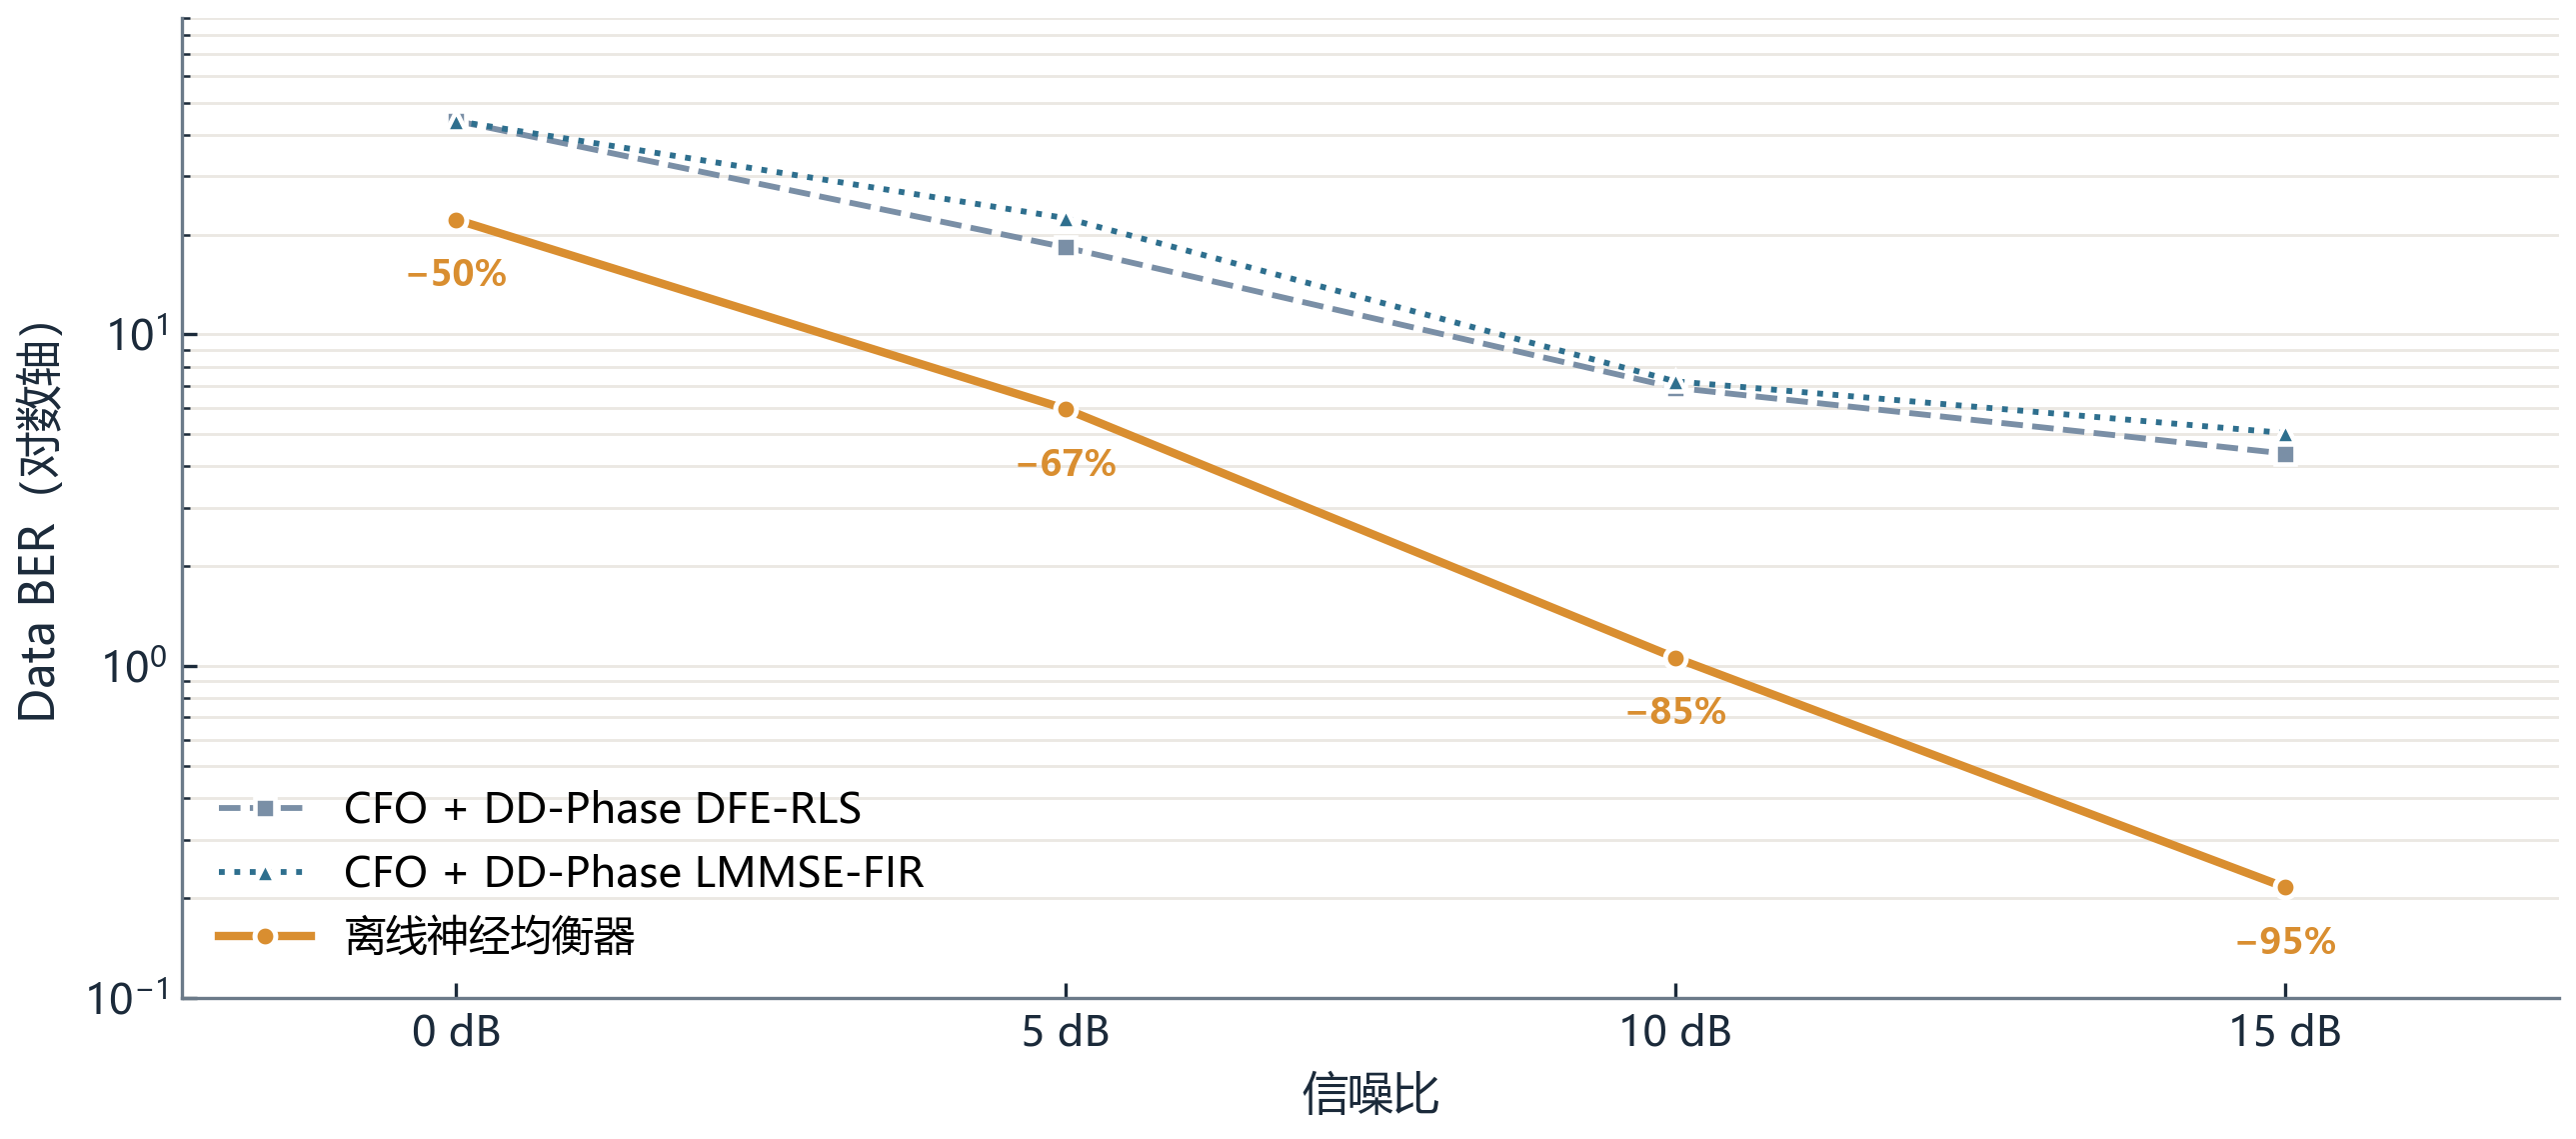
\includegraphics[width=0.95\linewidth]{figures/fig_offline_ber.png}
\caption{离线神经均衡器与传统均衡器在 3 seed × 60 帧主矩阵上的 Data BER。标注为相对 CFO+DD-Phase DFE-RLS 的 BER 降低比例。}
\end{figure}

这张表说明离线模型提供了强均衡起点，但它不是在线增益的证据。主矩阵的统计单位仍是独立 session；每个 SNR 只有 3 个 seed，不能把 180 帧当作 180 个独立样本来夸大显著性。本文的在线主张只与同源 Frozen 比较，见 6.2 节。

\subsection{独立确认的主效应与安全护栏}

表 2 与图 4 给出确认结果。四个 SNR 的 session 级配对增益均为正：0 dB $+0.036802$（SE $3.55\times10^{-3}$，单侧 95\% 下界 $+0.030289$），5 dB $+0.008032$（SE $9.64\times10^{-4}$，下界 $+0.006265$），10 dB $+0.001971$（SE $2.81\times10^{-4}$，下界 $+0.001456$），15 dB $+0.000260$（SE $6.06\times10^{-5}$，下界 $+0.000149$）。Holm 校正后的 $p$ 值分别为 $1\times10^{-5}$、$2\times10^{-5}$、$6\times10^{-5}$、$1\times10^{-3}$；每个 SNR 均为 0/10 个负向 session。H1 的四 SNR 等权平均增益为 $+0.011767$（SE $8.61\times10^{-4}$，单侧下界 $+0.010188$，$p=1.26\times10^{-7}$）。H2 在四个 SNR 上均通过。

\begin{table}[htbp]
\centering
\small
\caption{独立确认 v1 的逐 SNR 配对结果。ΔBER 定义为 $\mathrm{BER}_{\mathrm{frozen}}-\mathrm{BER}_{\mathrm{bayes}}$；下界为单侧 95\% $t$ 下界（df=9）。}
\begin{tabular}{lrrrrrrr}
\toprule
SNR & Frozen BER & Bayes BER & ΔBER & SE & 单侧 95\% 下界 & Holm $p$ & 负向 session \\
\midrule
0 dB & 0.2081 & 0.1713 & +0.036802 & $3.55\times10^{-3}$ & +0.030289 & $1\times10^{-5}$ & 0/10 \\
5 dB & 0.0479 & 0.0399 & +0.008032 & $9.64\times10^{-4}$ & +0.006265 & $2\times10^{-5}$ & 0/10 \\
10 dB & 0.00623 & 0.00426 & +0.001971 & $2.81\times10^{-4}$ & +0.001456 & $6\times10^{-5}$ & 0/10 \\
15 dB & 0.000985 & 0.000724 & +0.000260 & $6.06\times10^{-5}$ & +0.000149 & $1\times10^{-3}$ & 0/10 \\
\bottomrule
\end{tabular}
\end{table}

\begin{figure}[htbp]
\centering
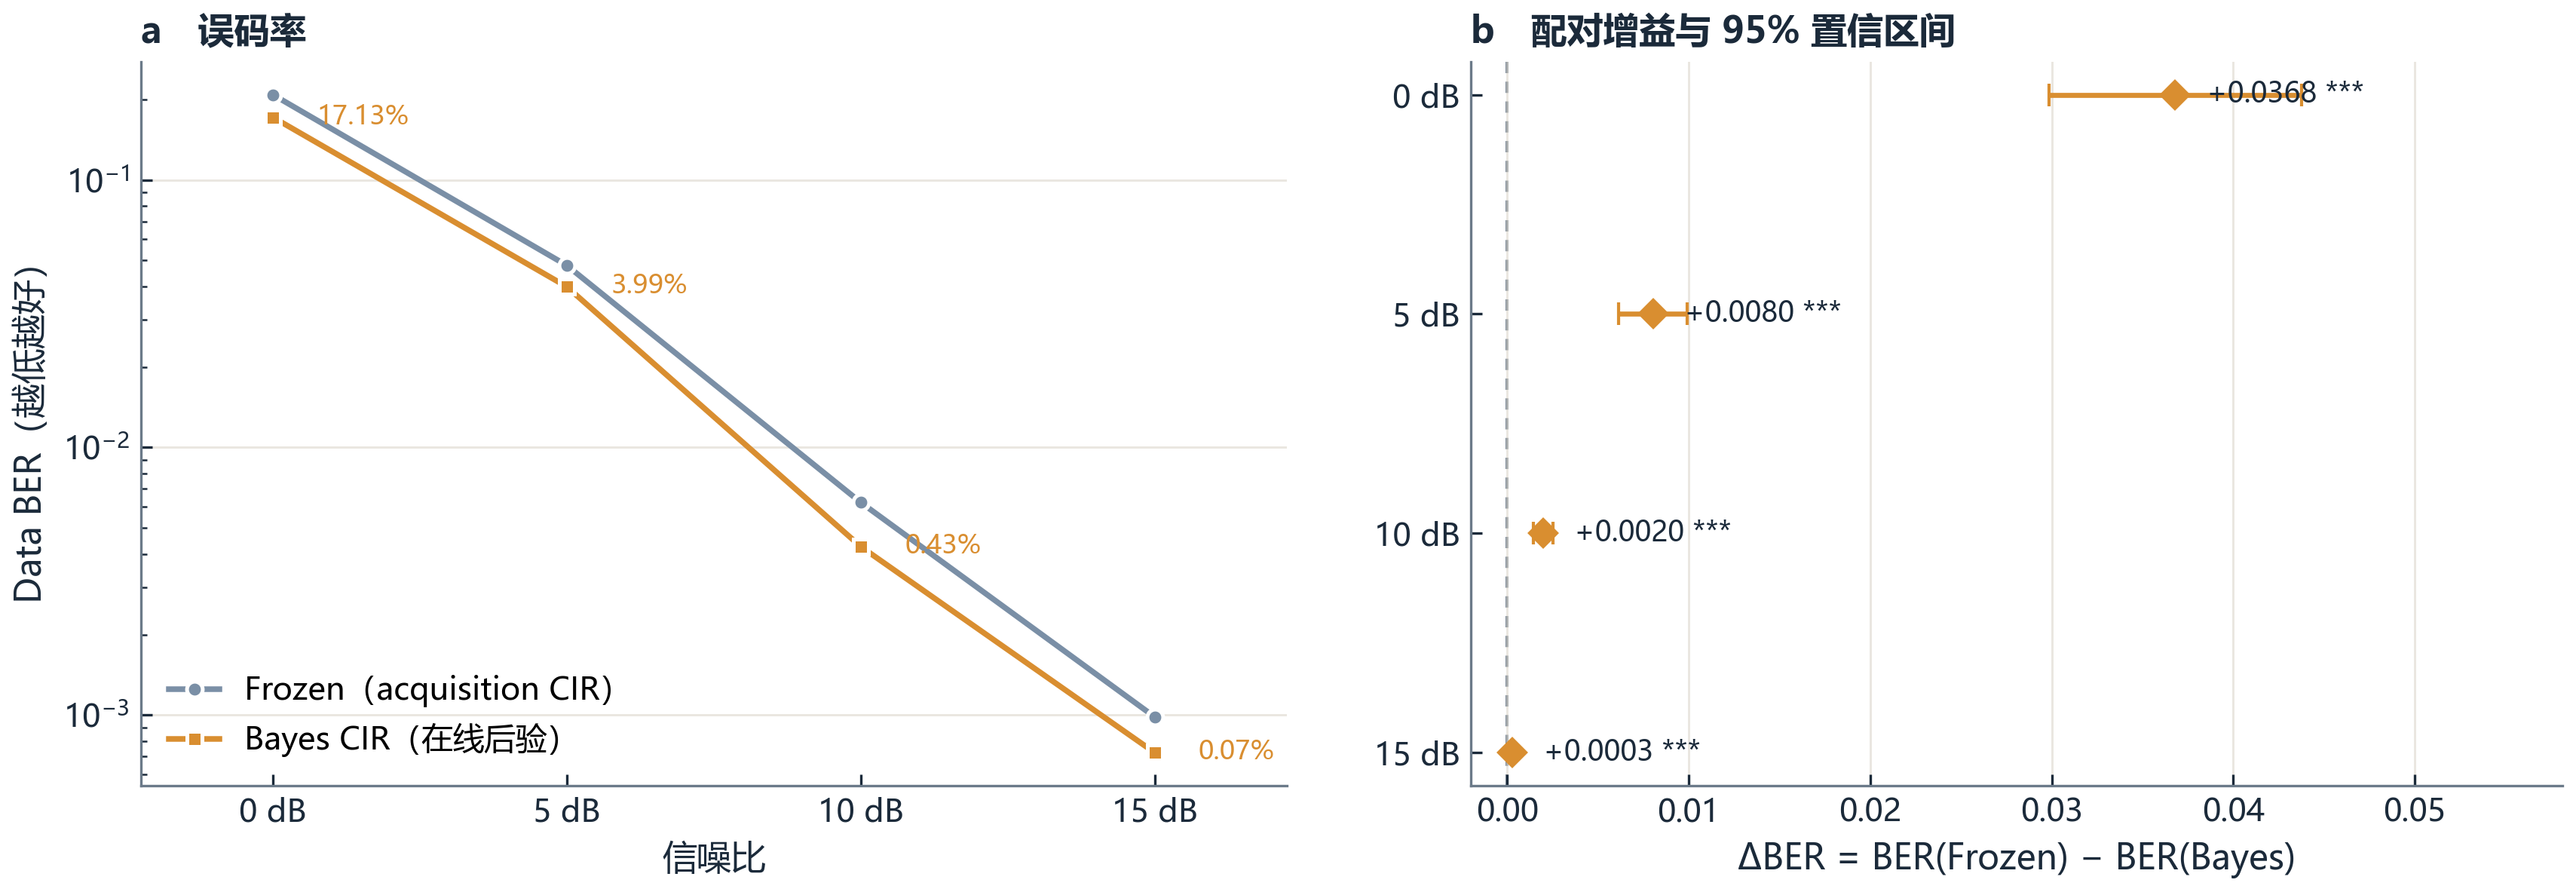
\includegraphics[width=0.95\linewidth]{figures/fig_ber_forest.png}
\caption{独立确认 v1 的 BER 曲线与逐 SNR 配对增益森林图。左：Frozen 与 Bayes 的四 SNR 平均 BER；右：session 级配对 ΔBER 与双侧 95\% 置信区间（1.96×SE）。}
\end{figure}

这里的下界是单侧 95\% $t$ 下界（df=9）；图 4b 画的是双侧 95\% 区间（$1.96\times\mathrm{SE}$），两者口径不同，但都远离零。需要强调，0 dB 的绝对 BER 仍为 17.13\%，远高于 5 dB 的 3.99\%；增益显著不等于链路可用。本文报告的是相对同源 Frozen 的改善，而不是绝对性能承诺。把 ΔBER 换成净错误数可以避免过度解读。在 128 帧 × 768 bit 的 session 上，0 dB 的增益远大于单个 bit 的偶然翻转；15 dB 的效应虽小，但仍对应可计数的净错误，而不是一个 bit 的噪声。本文在报告均值的同时保留逐 session 分布，原因正在于此。

\subsection{会话级一致性}

图 5 给出 10 个 session 的配对增益分布。四个 SNR 的 10 个点全部位于零线以上，没有负向 session；0 dB 的 session 间散布最大，5/10/15 dB 逐渐收紧。0 dB 的单 session 增益范围较宽，这与该 SNR 的深衰落和错误传播一致；但 10 个 session 的均值仍远离零，单侧下界为 $+0.0303$。5 dB 的均值 $+0.0080$、下界 $+0.0063$；10 dB 的均值 $+0.0020$、下界 $+0.0015$；15 dB 的均值 $+0.00026$、下界 $+0.00015$。后两个 SNR 的效应绝对值很小，但在配对设计和 10 个 session 下仍可分辨。

\begin{figure}[htbp]
\centering
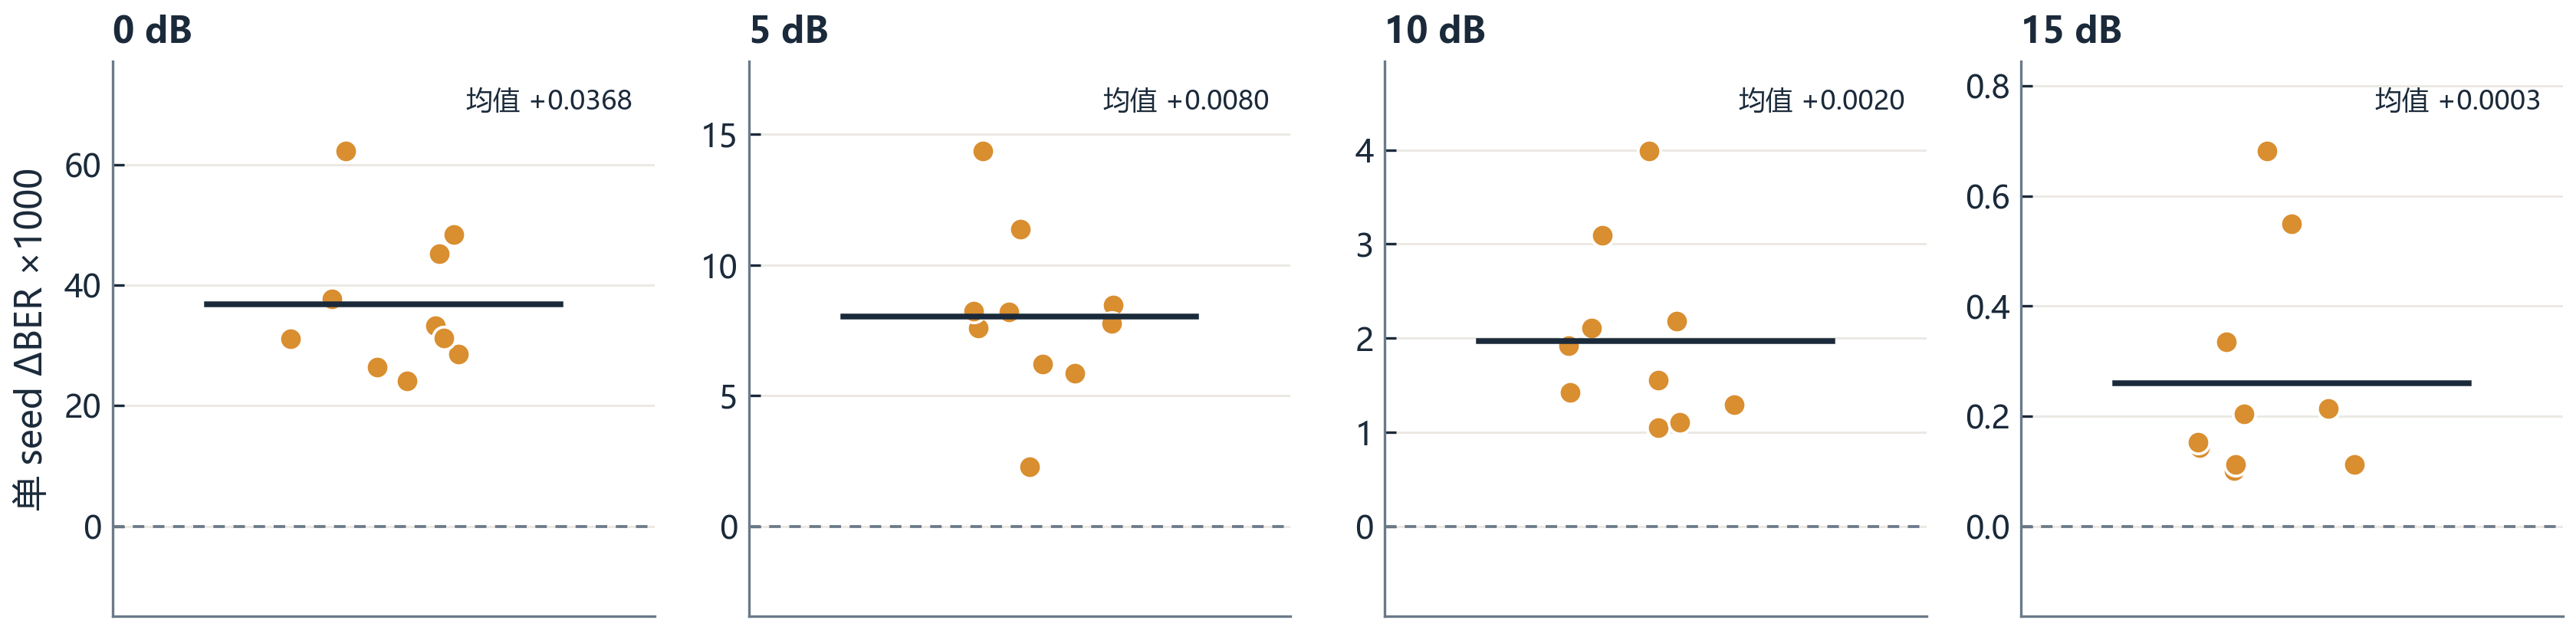
\includegraphics[width=0.95\linewidth]{figures/fig_seed.png}
\caption{10 个独立 session 的配对增益分布。每个点为一个 session 的 ΔBER；横线为 10 session 均值。}
\end{figure}

\subsection{增益随帧演化}

表 3 与图 6 给出 16 帧窗口的配对增益。5 dB 的窗口从 $+0.0058$ 上升到 $+0.0097$，斜率 $+0.000410$/bin；10 dB 从 $+0.00055$ 上升到 $+0.00335$，斜率 $+0.000377$/bin；15 dB 从 $+0.00005$ 上升到 $+0.00053$，斜率 $+0.000064$/bin；三者均满足 H3。0 dB 的窗口为 $+0.0267$、$+0.0587$、$+0.0502$、$+0.0416$、$+0.0160$、$+0.0134$、$+0.0513$、$+0.0365$，斜率 $-0.001238$/bin；末窗减首窗为 $+0.0098$，但由于第 2 窗的早期峰值，斜率仍为负。按预注册判据，H3 在 0 dB 不通过。

\begin{table}[htbp]
\centering
\small
\caption{独立确认 v1 的 16 帧窗口增益与会话级斜率。H3 要求斜率与末窗减首窗均为正；0 dB 的末窗减首窗为正，但斜率因第 2 窗早期峰值而为负。}
\begin{tabular}{lrrrr}
\toprule
SNR & 16 帧窗口增益（Frozen−Bayes） & 斜率/bin & 首窗 / 末窗 & H3 \\
\midrule
0 dB & +0.0267, +0.0587, +0.0502, +0.0416, +0.0160, +0.0134, +0.0513, +0.0365 & −0.001238 & +0.0267 / +0.0365 & 不通过 \\
5 dB & +0.0058, +0.0059, +0.0067, +0.0129, +0.0067, +0.0097, +0.0068, +0.0097 & +0.000410 & +0.0058 / +0.0097 & 通过 \\
10 dB & +0.00055, +0.00112, +0.00146, +0.00195, +0.00180, +0.00278, +0.00276, +0.00335 & +0.000377 & +0.00055 / +0.00335 & 通过 \\
15 dB & +0.00005, +0.00009, +0.00029, +0.00014, +0.00017, +0.00037, +0.00044, +0.00053 & +0.000064 & +0.00005 / +0.00053 & 通过 \\
\bottomrule
\end{tabular}
\end{table}

\begin{figure}[htbp]
\centering
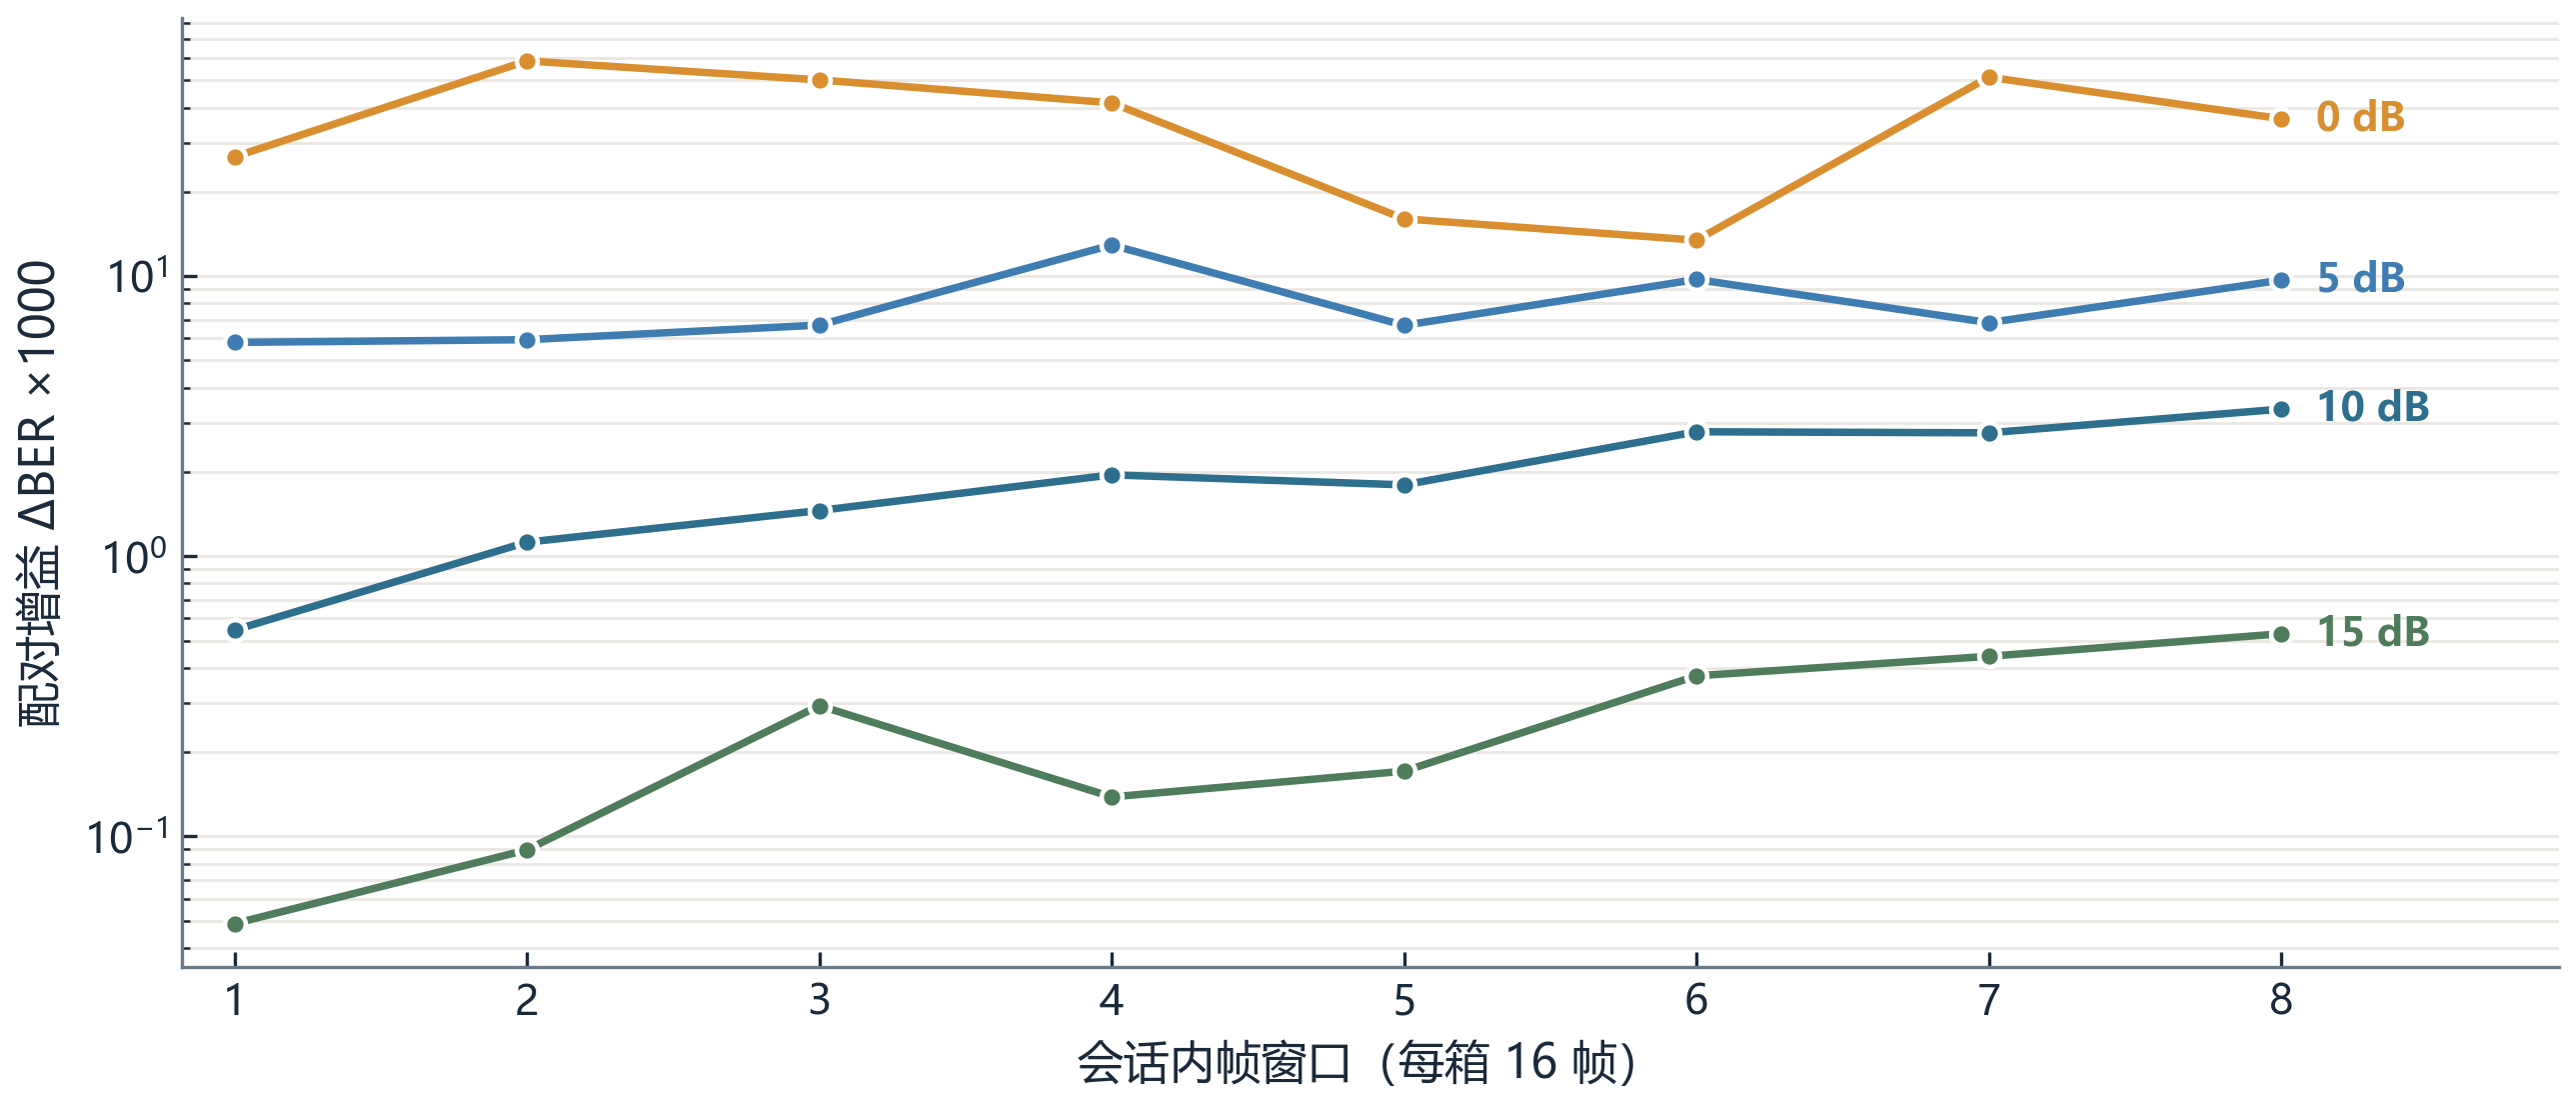
\includegraphics[width=0.95\linewidth]{figures/fig_growth.png}
\caption{配对增益随会话内帧窗口的演化。每箱 16 帧；0 dB 呈早期峰值后波动，5/10/15 dB 总体上升。}
\end{figure}

0 dB 的形状应描述为“早期收敛、随后波动/饱和、晚窗仍为正”，而不是“随帧增长”。四 SNR 平均 $+0.011767$ 不能用来掩盖这一点；本文在摘要、结果与结论中都单独报告 0 dB 的 H3 失败。5/10/15 dB 的增长与“后验协方差随帧收缩、过程噪声设定稳态”的解释一致；0 dB 的早期峰值则提示低 SNR 下的软判决后验在最初几帧快速吸收信息，随后被错误传播与信道波动主导。0 dB 的失败不是符号错误，而是形状错误：增益的符号在 10/10 session 上一致为正，但窗口斜率因早期峰值而为负。若只看末窗减首窗，会误以为 0 dB 也满足增长；预注册判据同时要求斜率与末窗减首窗为正，正是为了防止这种选择性解读。

\subsection{CIR 估计误差}

表 4 与图 7 给出 CIR 的 NMSE。Frozen 的 NMSE 为 0.1317/0.0520/0.0233/0.0141，Bayes 为 0.0383/0.0173/0.0065/0.0035；四个 SNR 分别下降约 71\%、67\%、72\%、75\%，整体在 67\%–75\% 之间。这与 6.2 的 BER 增益方向一致：0 dB 的 NMSE 绝对下降最大（0.1317→0.0383），其 BER 增益也最大；10/15 dB 的 NMSE 绝对下降较小，BER 增益也较小。

\begin{table}[htbp]
\centering
\small
\caption{Frozen 与 Bayes 的 CIR 归一化均方误差。下降比例由表中数值计算。}
\begin{tabular}{lrrr}
\toprule
SNR & Frozen NMSE & Bayes NMSE & 下降 \\
\midrule
0 dB & 0.1317 & 0.0383 & 70.9\% \\
5 dB & 0.0520 & 0.0173 & 66.7\% \\
10 dB & 0.0233 & 0.0065 & 72.1\% \\
15 dB & 0.0141 & 0.0035 & 75.2\% \\
\bottomrule
\end{tabular}
\end{table}

\begin{figure}[htbp]
\centering
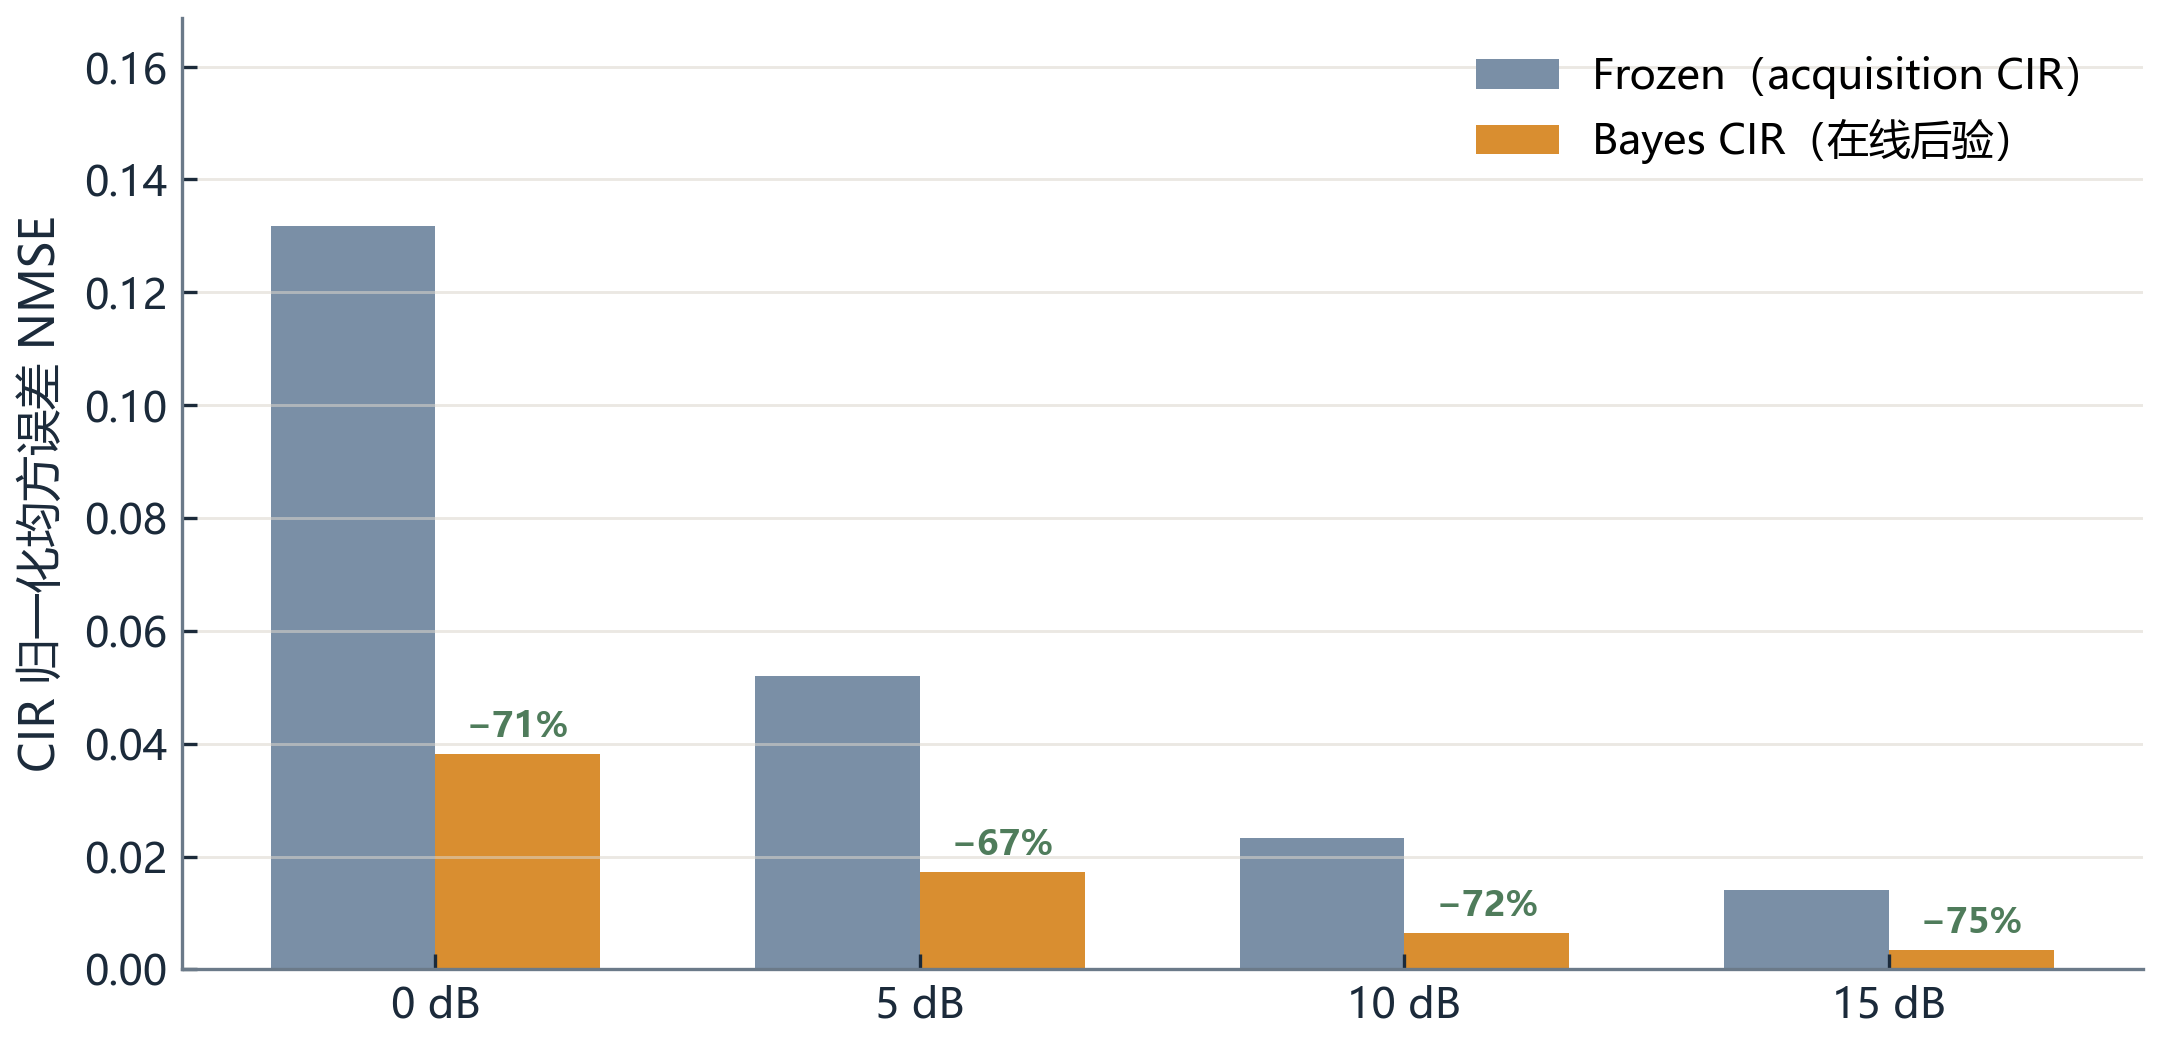
\includegraphics[width=0.95\linewidth]{figures/fig_nmse.png}
\caption{Frozen 与 Bayes 的 CIR 估计 NMSE。标注为相对 Frozen 的下降比例。}
\end{figure}

NMSE 不是本文的主判据，但它提供了机制证据：Bayes 与 Frozen 的唯一差异是 CIR 后验，NMSE 的下降说明后验确实在跟踪信道，而不是通过其他路径改变判决。真实 CIR 只用于离线 oracle 诊断，不进入在线分支。

\subsection{开发规模一致性}

图 8 与表 5 汇总三种开发规模：5×32、10×64、10×128。5/10 dB 的增益在三种规模上均为正，且随规模增大保持同向；15 dB 从 5×32 的中性（$+0.000033$）增长到 10×64 的 $+0.00013$、10×128 的 $+0.00049$，说明长会话对高 SNR 的小效应更重要；0 dB 的点估计在 $+0.0223$ 到 $+0.0351$ 之间波动，主要由 session 间方差主导，但三种规模均为正。3×16 的开发筛查也给出 3/3 seed 同向（0 dB 点估计 $+0.0297$，5 dB $+0.00697$，10 dB $+0.00185$，15 dB 中性）。这些开发结果不能替代 10×128 的独立确认，但说明确认结果不是单一规模或单一 seed 族的偶然产物。开发规模的扩展还说明，0 dB 的点估计不稳定主要来自 session 方差，而不是机制方向改变：3×16、5×32、10×64、10×128 四组开发 seed 的符号均为正。5/10 dB 的点估计在四组开发 seed 上分别处于 $+0.0056$–$+0.0070$ 与 $+0.0014$–$+0.0022$ 之间，随规模增大没有反向；15 dB 的 5×32 点估计接近零，10×64 与 10×128 才给出可辨认的正增益。

\begin{table}[htbp]
\centering
\small
\caption{不同开发规模上的 session 级配对增益。区间与逐 seed 细节见开发归档；这些 seed 不并入确认。}
\begin{tabular}{lrrrrr}
\toprule
规模 & seed & 0 dB & 5 dB & 10 dB & 15 dB \\
\midrule
3×16 & 95001–95003 & +0.0297（3/3 同向） & +0.00697 & +0.00185 & 中性 \\
5×32 & 97001–97005 & +0.0318 & +0.00561 & +0.00141 & 中性 \\
10×64 & 98001–98010 & +0.0351 & +0.00575 & +0.00155 & +0.00013 \\
10×128 & 99001–99010 & +0.0223 & +0.00615 & +0.00220 & +0.00049 \\
\bottomrule
\end{tabular}
\end{table}

\begin{figure}[htbp]
\centering
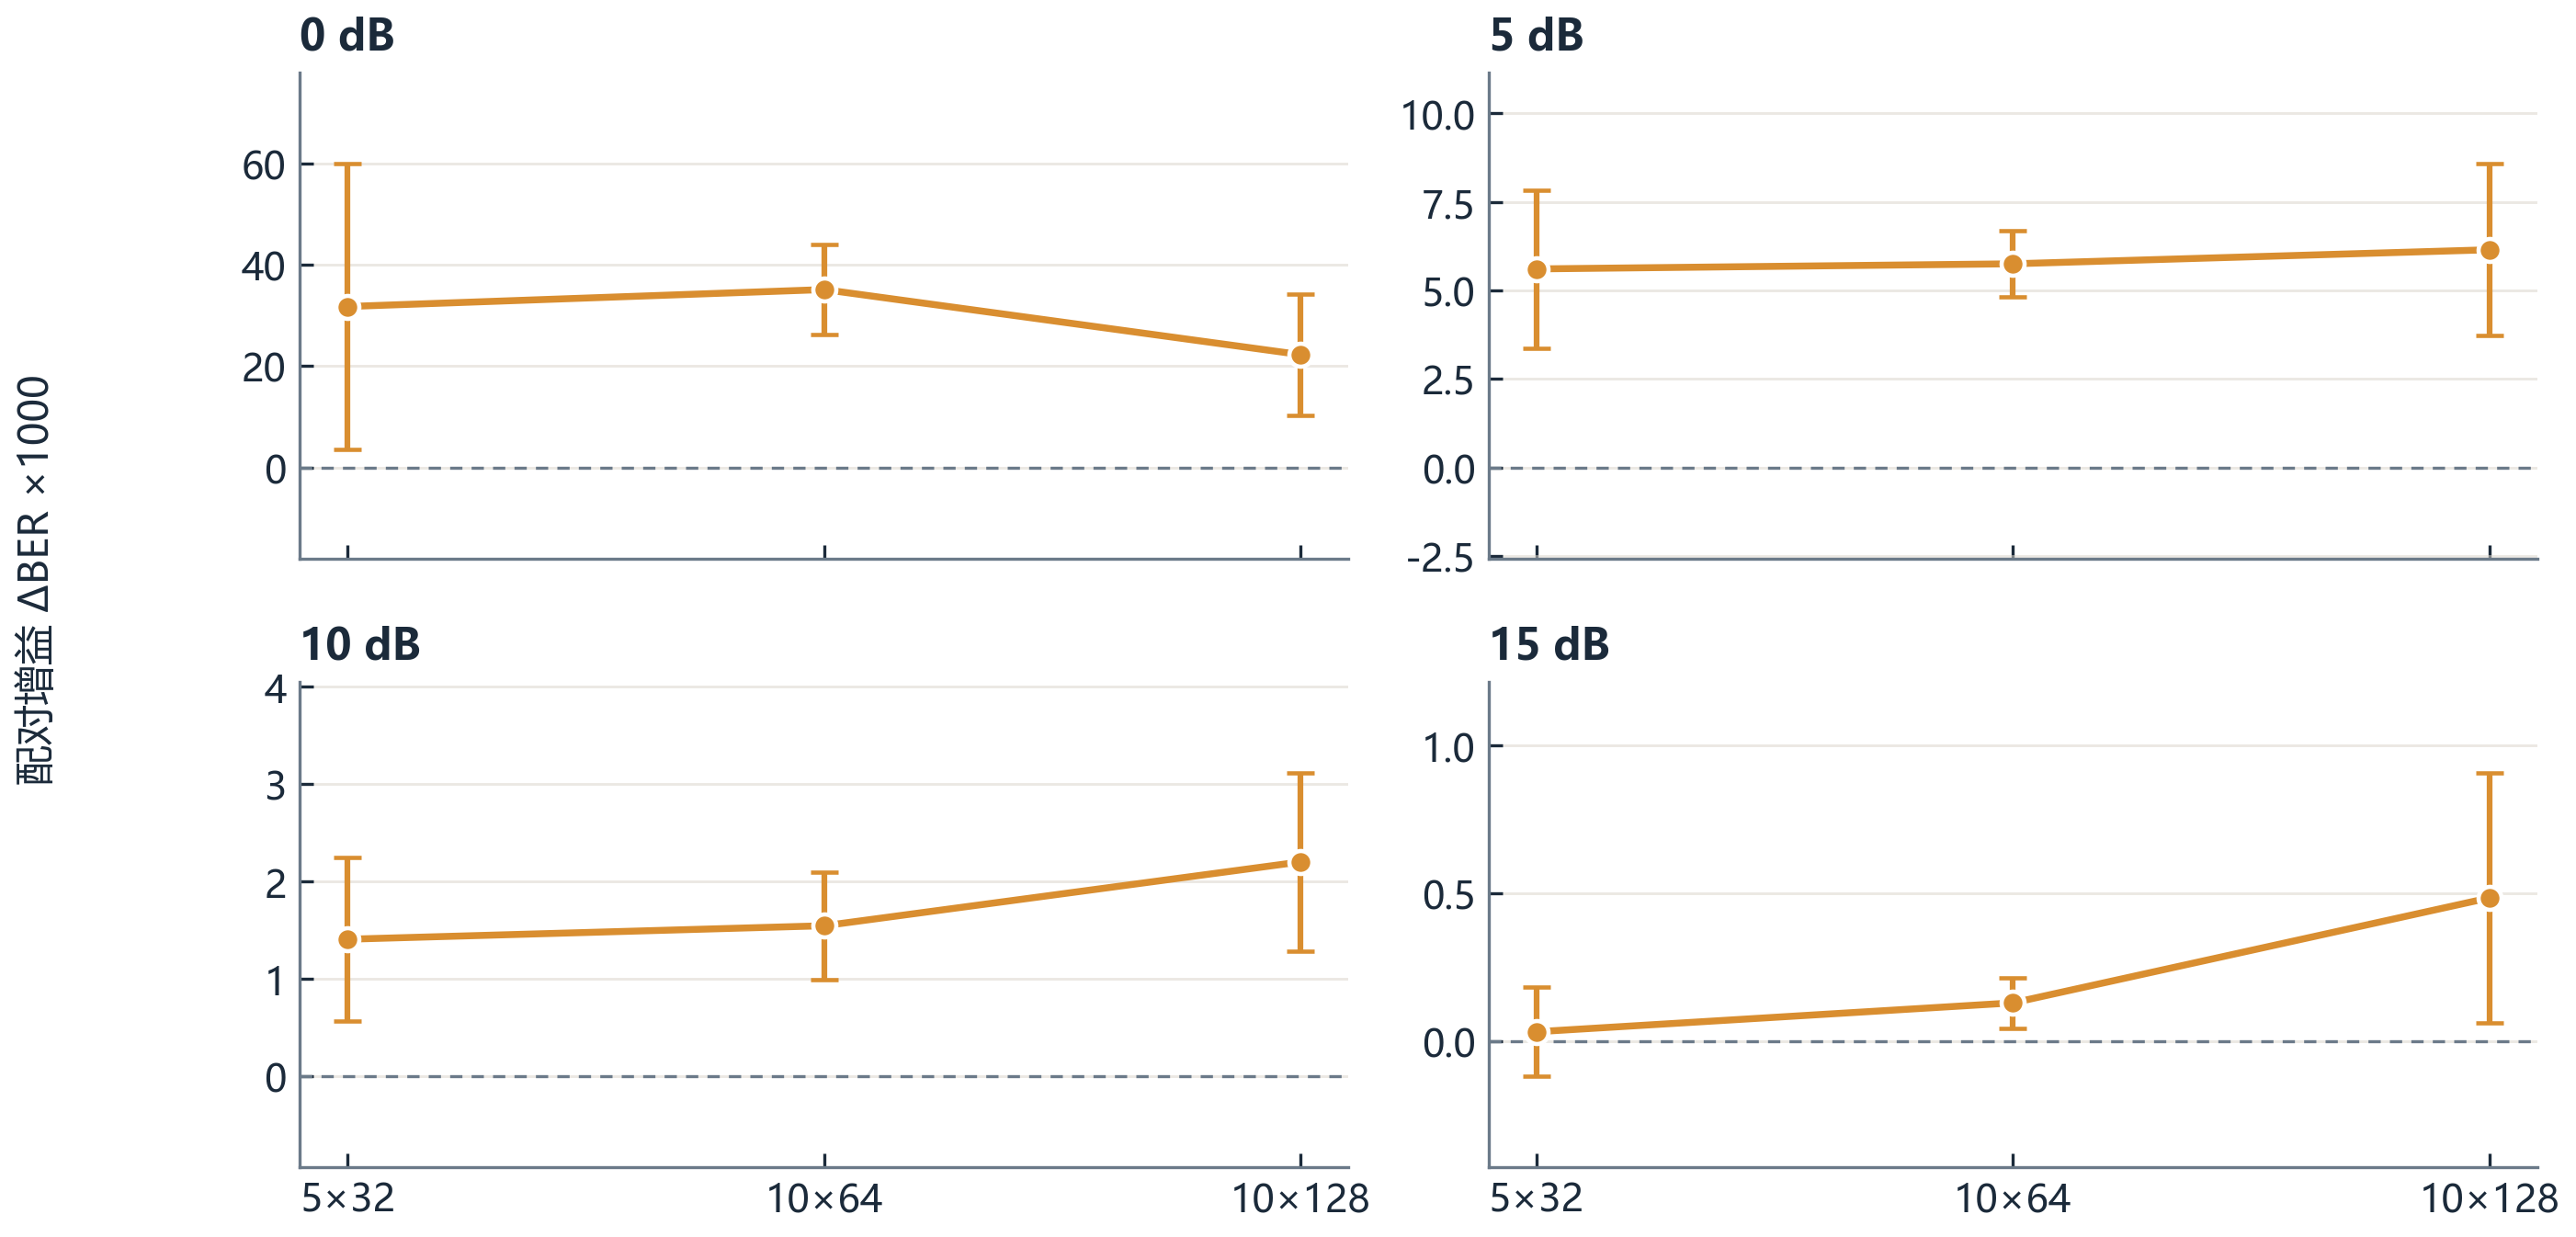
\includegraphics[width=0.95\linewidth]{figures/fig_scale.png}
\caption{三种开发规模（5×32、10×64、10×128）上的配对增益一致性。误差棒为描述性 95\% 区间。}
\end{figure}

\subsection{与传统接收机的公平对照}

为判断物理增益是否只是在弱基线上有效，本文在 3 seed × 16 帧的开发对照中（seed 130001–130003），把 Frozen/Bayes 与同波形、同 Pilot 预算、同 acquisition CIR 的传统接收机比较。0 dB 的 Data BER：Bayes 18.14\%、Frozen 21.46\%、CFO+DD-Phase LMMSE-FIR 43.66\%、DFE-RLS 40.64\%、SC-FDE-MMSE 49.06\%；10 dB：Bayes 0.727\%、Frozen 0.814\%、LMMSE-FIR 4.13\%、DFE-RLS 3.59\%、SC-FDE-MMSE 48.42\%。传统接收机不读 Reward/Data 标签，也不使用神经网络或强化学习；逐 (seed, frame) 配对差（传统−Bayes、传统−Frozen）全部为正，每个 SNR 48 对。SC-FDE-MMSE 未做 CFO/相位补偿，接近随机，只作弱对照。该对照是开发规模，不是确认级证据；它说明本文的起点不是弱基线，但传统方法的确认级比较仍需更大样本。公平性检查包括：同帧接收波形哈希一致、Frozen 与传统方法共享同一 acquisition CIR、传统方法 \texttt{uses\_neural\_network=False}、\texttt{uses\_reward\_or\_data\_labels=False}。这些检查排除了传统基线通过读取标签或使用不同波形获得优势的可能。
